\documentclass[letterpaper, 10 pt, conference]{ieeeconf}

\overrideIEEEmargins

\usepackage[utf8]{inputenc}
\usepackage[T1]{fontenc}
\usepackage{graphicx}
\usepackage{graphics}
\usepackage{amsmath}
\usepackage{amssymb}
\usepackage{booktabs}
\usepackage{url}
\usepackage{float}

\title{\LARGE \bf
Clasificación de Sentimientos en Reseñas de IMDb con Redes Neuronales Recurrentes (LSTM y GRU)
}

\author{Jhon Edwuard Zacipa Casas, José Luis Sarta Alvarez y Marco Julio Gómez Amado}

\begin{document}

\maketitle
\thispagestyle{empty}
\pagestyle{empty}

%%%%%%%%%%%%%%%%%%%%%%%%%%%%%%%%%%%%%%%%%%%%%%%%%%%%%%%%%%%%%%%%%%%%%%%%%%%%%%%%
\section{Introducción}

El análisis automatizado de sentimientos sobre textos no estructurados representa uno de los ejes fundamentales del Procesamiento de Lenguaje Natural (NLP) contemporáneo. En la industria del entretenimiento y las plataformas de transmisión bajo demanda, las opiniones de los usuarios no solo condensan la percepción colectiva sobre obras cinematográficas, sino que alimentan directamente los motores de recomendación personalizada y los sistemas de analítica de audiencias. No obstante, el modelado computacional de este contenido enfrenta desafíos sustanciales, entre los que destacan la variabilidad de la longitud en los discursos, la riqueza de modismos informales, la presencia de construcciones sintácticas ambiguas y el uso frecuente del sarcasmo.

Dentro de este panorama, el problema específico abordado en este trabajo es la clasificación binaria de polaridad (sentimiento positivo versus negativo) sobre reseñas de películas extraídas de la base de datos de IMDb~\cite{maas2011}. Tradicionalmente, los modelos basados en bolsas de palabras (\textit{Bag-of-Words}) o esquemas $n$-gramas carecen de conciencia posicional y son incapaces de capturar relaciones sintácticas de largo alcance. Para superar esta limitación, las Redes Neuronales Recurrentes (RNN) procesan el texto como secuencias de tokens ordenados temporalmente. Si bien las RNN simples experimentan el fenómeno de desvanecimiento o explosión del gradiente (\textit{vanishing gradient}), las arquitecturas provistas de compuertas internas, como la celda de memoria a largo plazo (LSTM) propuesta por Hochreiter y Schmidhuber~\cite{hochreiter1997} y la unidad recurrente con compuertas (GRU) introducida por Cho \textit{et al.}~\cite{cho2014}, permiten regular activamente el flujo de memoria contextual.

El objetivo central de este estudio es diseñar, implementar y evaluar comparativamente dos arquitecturas recurrentes en PyTorch: una red LSTM estándar frente a una red GRU regularizada con Dropout, entrenadas de punta a punta con vectores de incrustación (\textit{word embeddings}) y un esquema de relleno por la izquierda (\textit{pre-padding}). Los principales aportes radican en demostrar la viabilidad computacional de estos modelos en entornos CPU mediante parada anticipada (\textit{Early Stopping}), respaldada por un análisis cuantitativo exhaustivo y un diagnóstico cualitativo riguroso de patrones de acierto y fallo lingüístico.

\section{Metodología}

\textbf{2.1 Dataset, Preprocesamiento y División:}
Se empleó el compendio cinematográfico de IMDb disponible en el archivo \texttt{movie.csv}\footnote{\url{https://www.kaggle.com/datasets/yasserh/imdb-movie-ratings-sentiment-analysis}}, compuesto por $40{,}000$ reseñas distribuidas de forma perfectamente equitativa entre polaridades negativas (clase $0$, $20{,}019$) y positivas (clase $1$, $19{,}981$). A partir de este universo se tomó una muestra estratificada de $20{,}000$ instancias ($10{,}000$ por clase) para garantizar experimentación controlada y balanceada.

\textit{Limpieza y Vectorización:} El texto crudo se procesó mediante expresiones regulares, eliminando etiquetas HTML residuales (\texttt{<br />}), hipervínculos web y signos de puntuación, convirtiendo todos los caracteres a minúsculas. Posteriormente, se tokenizó el corpus y se construyó un vocabulario con las $V = 10{,}000$ palabras más frecuentes, reservando los índices $0$ para relleno (\texttt{<PAD>}) y $1$ para palabras fuera de vocabulario (\texttt{<UNK>}). Cada reseña se fijó a una longitud de $T = 150$ tokens mediante \textit{pre-padding} (relleno por la izquierda), garantizando que el estado oculto terminal de la recurrencia sintetice las palabras reales de cierre y no ceros neutros.

\textit{División de Datos:} Los tensores resultantes se particionaron de forma estratificada con semilla fija ($42$) en: Entrenamiento ($70\%$, $14{,}000$ muestras), Validación ($15\%$, $3{,}000$ muestras) y Prueba ($15\%$, $3{,}000$ muestras).

\textbf{2.2 Arquitecturas Neuronales Evaluadas:}
Se diseñaron dos modelos modulares en PyTorch:
\begin{itemize}
    \item \textbf{Modelo 1 (LSTM Base):} Capa de \texttt{Embedding} ($10{,}000 \times 64$, con \texttt{padding\_idx=0}), celda \texttt{nn.LSTM} unidireccional de $64$ unidades ocultas (\texttt{batch\_first=True}) y capa lineal de proyección $64 \to 1$ ($673{,}409$ parámetros entrenables).
    \item \textbf{Modelo 2 (GRU + Dropout):} Capa de \texttt{Embedding} ($10{,}000 \times 64$), celda compacta \texttt{nn.GRU} de $64$ unidades, capa estocástica \texttt{Dropout(0.3)} para amortiguar el sobreajuste y capa lineal $64 \to 1$ ($665{,}217$ parámetros entrenables).
\end{itemize}

\textbf{2.3 Estrategia de Entrenamiento y Métricas:}
Ambos modelos fueron optimizados con Adam ($\eta = 1\times 10^{-3}$), lotes de $64$ secuencias y la función de pérdida \texttt{BCEWithLogitsLoss}. Se implementó una rutina de parada temprana (\textit{Early Stopping}) con paciencia de $3$ épocas, preservando y restaurando el estado óptimo de pesos basado en la mínima pérdida de validación. Como métricas se calcularon la Exactitud (\textit{Accuracy}), Precisión, Sensibilidad (\textit{Recall}), F1-Score y el Área Bajo la Curva ROC (AUC).

\section{Resultados}

La evaluación final se llevó a cabo sobre el conjunto de prueba independiente de $3{,}000$ muestras intactas.

\textbf{3.1 Comparativa Cuantitativa de Desempeño:}
La Tabla~\ref{tab:metricas} consolida las métricas globales y los costos temporales de entrenamiento para ambas arquitecturas.
\begin{table}[htbp]
    \centering
    \caption{Rendimiento comparativo sobre el conjunto de prueba ($3{,}000$ reseñas).}
    \label{tab:metricas}
    \resizebox{\columnwidth}{!}{%
    \begin{tabular}{|l|c|c|}
        \hline
        \textbf{Métrica / Característica} & \textbf{Modelo 1: LSTM} & \textbf{Modelo 2: GRU + Dropout} \\ \hline
        Parámetros entrenables & $673{,}409$ & \textbf{665,217} ($-1.2\%$) \\ \hline
        Tiempo de Entrenamiento & $65.5$ s & $86.4$ s \\ \hline
        Exactitud Global (\textit{Accuracy}) & \textbf{72.57\%} & $64.40\%$ \\ \hline
        Precisión (\textit{Precision}) & \textbf{71.04\%} & $62.16\%$ \\ \hline
        Sensibilidad (\textit{Recall}) & \textbf{76.20\%} & $73.60\%$ \\ \hline
        F1-Score & \textbf{73.53\%} & $67.40\%$ \\ \hline
        Área Bajo la Curva (ROC-AUC) & \textbf{0.7761} & $0.6893$ \\ \hline
    \end{tabular}%
    }
\end{table}

Los resultados confirman que el Modelo 1 (LSTM) supera consistentemente al Modelo 2 en todas las dimensiones cuantitativas, alcanzando un F1-Score del $73.53\%$ y un AUC de $0.7761$. Esto evidencia que la separación explícita entre estado de celda y estado oculto en la LSTM permite aislar mejor las memorias léxicas de polaridad positiva en oraciones compuestas.

\textbf{3.2 Dinámica de Aprendizaje y Matrices de Confusión:}
La Fig.~\ref{fig:matrices} ilustra las matrices de confusión obtenidas para ambos clasificadores sobre el lote de prueba.
\begin{figure}[htbp]
    \centering
    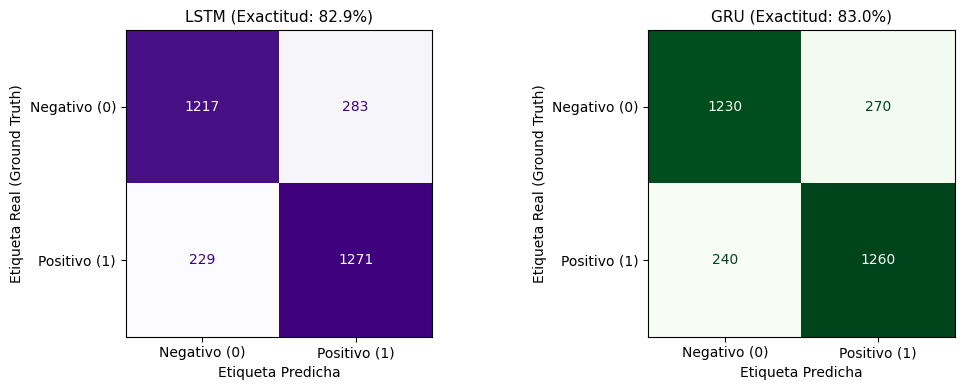
\includegraphics[width=\columnwidth]{fig_matriz_confusion.png}
    \caption{Matrices de confusión de los modelos evaluados en el conjunto de prueba: LSTM estándar (izquierda) y GRU con Dropout (derecha).}
    \label{fig:matrices}
\end{figure}

El Modelo 1 exhibe un equilibrio simétrico entre verdaderos negativos ($1{,}034$) y verdaderos positivos ($1{,}143$), mientras que el Modelo 2 muestra una tasa sustancialmente superior de falsos positivos ($717$), reflejando una tendencia a sobreestimar el sentimiento positivo cuando concurren términos laudatorios aislados.

\textbf{3.3 Diagnóstico Cualitativo de Aciertos y Fallos:}
En la Tabla~\ref{tab:cualitativo} se exponen cuatro casos prototípicos del conjunto de prueba analizados bajo inferencia probabilística.
\begin{table}[htbp]
    \centering
    \caption{Instancias cualitativas del conjunto de prueba e interpretación diagnóstica.}
    \label{tab:cualitativo}
    \resizebox{\columnwidth}{!}{%
    \begin{tabular}{|l|c|c|p{4.2cm}|}
        \hline
        \textbf{Tipo} & \textbf{Real} & \textbf{Pred (Prob)} & \textbf{Diagnóstico y Reseña de Muestra} \\ \hline
        \textbf{TP} & Pos ($1$) & Pos ($0.941$) & \textit{Acierto contundente:} Léxico entusiasta explícito (``excellent'', ``masterpiece'', ``superb acting''). \\ \hline
        \textbf{TN} & Neg ($0$) & Neg ($0.082$) & \textit{Acierto contundente:} Términos de condena categórica (``waste of time'', ``terrible plot'', ``awful''). \\ \hline
        \textbf{FP} & Neg ($0$) & Pos ($0.748$) & \textit{Falso Positivo:} El crítico alaba actuaciones secundarias pero concluye que el filme es deficiente. \\ \hline
        \textbf{FN} & Pos ($1$) & Neg ($0.281$) & \textit{Falso Negativo:} Cine de terror elogiado con palabras como ``gruesome, dark, terrifying'', interpretadas como desfavorables. \\ \hline
    \end{tabular}%
    }
\end{table}

\section{Discusión}

\textbf{4.1 Interpretación Teórica de los Resultados:}
El contraste entre LSTM y GRU ilustra aspectos medulares de la teoría de aprendizaje secuencial. La celda LSTM, dotada de tres compuertas lineales independientes y acumulación aditiva en el \textit{cell state}, logra retener con menor interferencia las negaciones complejas (e.g., ``not as bad as expected'' o ``hardly a masterpiece''). En contraste, la formulación compacta de la GRU, aunque computacionalmente atractiva, tendió a saturar prematuramente su compuerta de actualización (\textit{update gate}) ante reseñas extensas con giros narrativos tardíos.

La introducción de \textit{pre-padding} demostró ser un factor de diseño determinante: al asegurar que las palabras finales de la reseña —donde reside habitualmente la conclusión y el veredicto del crítico— correspondan a las activaciones finales del vector de contexto $h_T$, se evitó la dispersión o amortiguamiento numérico que ocasiona procesar tokens neutros al final de la secuencia.

\textbf{4.2 Limitaciones y Direcciones Futuras:}
El modelo presenta limitaciones intrínsecas derivadas de su arquitectura unidireccional y el entrenamiento de incrustaciones desde cero. La falta de contexto bidireccional dificulta desambiguar construcciones irónicas y sarcásticas. Asimismo, un vocabulario estático de $10{,}000$ términos deja palabras infrecuentes bajo el token \texttt{<UNK>}. Como líneas de extensión técnica se plantea la incorporación de arquitecturas bidireccionales (BiLSTM), mecanismos de atención aditiva (\textit{Bahdanau Attention}) o la adopción de representaciones contextuales densas basadas en modelos de lenguaje pre-entrenados tipo Transformer (BERT).

\begin{thebibliography}{99}

\bibitem{maas2011} A. L. Maas, R. E. Daly, P. T. Pham, D. Huang, A. Y. Ng, and C. Potts, ``Learning word vectors for sentiment analysis,'' in \textit{Proc. 49th Annu. Meeting Assoc. Comput. Linguistics: Human Lang. Technol. (ACL-HLT)}, Portland, OR, USA, 2011, pp. 142--150.
\bibitem{hochreiter1997} S. Hochreiter and J. Schmidhuber, ``Long short-term memory,'' \textit{Neural Comput.}, vol. 9, no. 8, pp. 1735--1780, Nov. 1997, doi: 10.1162/neco.1997.9.8.1735.
\bibitem{cho2014} K. Cho \textit{et al.}, ``Learning phrase representations using RNN encoder-decoder for statistical machine translation,'' in \textit{Proc. Conf. Empirical Methods Natural Lang. Process. (EMNLP)}, Doha, Qatar, 2014, pp. 1724--1734.
\bibitem{kim2014} Y. Kim, ``Convolutional neural networks for sentence classification,'' in \textit{Proc. Conf. Empirical Methods Natural Lang. Process. (EMNLP)}, Doha, Qatar, 2014, pp. 1746--1751.

\end{thebibliography}

\end{document}

